\documentclass{scrreport}
\usepackage[ngerman]{babel}
\usepackage[utf8]{inputenc}
\usepackage[combine]{ucs}
\usepackage[pdftex]{graphicx}
\usepackage{listings} % source code formatting
\usepackage{blindtext}
\usepackage{wrapfig}
\usepackage{subfigure}
\usepackage{float}
\usepackage{subfiles}
\usepackage[numbers]{natbib}
\usepackage{fullpage}
\usepackage{hyperref}
\usepackage{courier}
\usepackage{color}
\usepackage[dvipsnames]{xcolor}
\usepackage{scrhack}
\usepackage{siunitx}
\usepackage{newfloat}
\DeclareFloatingEnvironment[
  fileext=lg,
  name=Code-Snippet,
  placement=htp,
]{code}
\bibliographystyle{unsrt}
\graphicspath{{images/}{../images/}} % set correct path to images
\headsep = 35pt

% Basic
\lstset{basicstyle=\ttfamily\scriptsize}
\lstset{showspaces=false}
\lstset{showtabs=false}
\lstset{showstringspaces=false}
\lstset{keywordstyle=\bfseries}
\lstset{tabsize=3}
\lstset{frameround=ffff}
\lstset{extendedchars=true}
\lstset{stringstyle=\ttfamily}
\lstset{commentstyle=\ttfamily}
\lstset{numbers=left, numberstyle=\tiny, stepnumber=1, numbersep=5pt}
\lstset{captionpos=b}
\lstset{frame=single}

% JavaScript
\definecolor{lightgray}{rgb}{.9,.9,.9}
\definecolor{darkgray}{rgb}{.4,.4,.4}
\definecolor{purple}{rgb}{0.65, 0.12, 0.82}
\lstdefinelanguage{JavaScript}{
  keywords={typeof, new, true, false, catch, function, return, null, catch, switch, const, var, let, if, in, while, do, else, case, break},
  keywordstyle=\color{blue}\bfseries,
  ndkeywords={string, number, class, export, boolean, throw, implements, import, this},
  ndkeywordstyle=\color{darkgray}\bfseries,
  identifierstyle=\color{black},
  sensitive=false,
  comment=[l]{//},
  morecomment=[s]{/*}{*/},
  commentstyle=\color{purple}\ttfamily,
  stringstyle=\color{red}\ttfamily,
  morestring=[b]',
  morestring=[b]"
}
\definecolor{codegreen}{rgb}{0,0.6,0}
\definecolor{codegray}{rgb}{0.5,0.5,0.5}
\definecolor{codepurple}{rgb}{0.58,0,0.82}
\definecolor{backcolour}{rgb}{0.95, 0.95, 0.96}
% Define the codebox
\lstset{
   language=JavaScript,
   backgroundcolor=\color{lightgray},
   extendedchars=true,
   basicstyle=\footnotesize\ttfamily,
   showstringspaces=false,
   showspaces=false,
   numbers=left,
   numberstyle=\footnotesize,
   numbersep=9pt,
   tabsize=2,
   breaklines=true,
   showtabs=false,
   captionpos=b
}
\DeclareOldFontCommand{\bf}{\normalfont\bfseries}{\mathbf}

%Rust
\definecolor{GrayCodeBlock}{RGB}{241,241,241}
\definecolor{BlackText}{RGB}{110,107,94}
\definecolor{RedTypename}{RGB}{182,86,17}
\definecolor{GreenString}{RGB}{96,172,57}
\definecolor{PurpleKeyword}{RGB}{184,84,212}
\definecolor{GrayComment}{RGB}{170,170,170}
\definecolor{GoldDocumentation}{RGB}{180,165,45}
\lstdefinelanguage{rust}
{
    columns=fullflexible,
    keepspaces=true,
    frame=single,
    framesep=0pt,
    framerule=0pt,
    framexleftmargin=4pt,
    framexrightmargin=4pt,
    framextopmargin=5pt,
    framexbottommargin=3pt,
    xleftmargin=4pt,
    xrightmargin=4pt,
    backgroundcolor=\color{GrayCodeBlock},
    basicstyle=\ttfamily\color{BlackText},
    numbers=none,
    keywords={
        true,false,
        unsafe,async,await,move,
        use,pub,crate,super,self,mod,
        struct,enum,fn,const,static,let,mut,ref,type,impl,dyn,trait,where,as,
        break,continue,if,else,while,for,loop,match,return,yield,in
    },
    keywordstyle=\color{PurpleKeyword},
    ndkeywords={
        bool,u8,u16,u32,u64,u128,i8,i16,i32,i64,i128,char,str,
        Self,Option,Some,None,Result,Ok,Err,String,Box,Vec,Rc,Arc,Cell,RefCell,HashMap,BTreeMap,
        macro_rules
    },
    ndkeywordstyle=\color{RedTypename},
    comment=[l][\color{GrayComment}\slshape]{//},
    morecomment=[s][\color{GrayComment}\slshape]{/*}{*/},
    morecomment=[l][\color{GoldDocumentation}\slshape]{///},
    morecomment=[s][\color{GoldDocumentation}\slshape]{/*!}{*/},
    morecomment=[l][\color{GoldDocumentation}\slshape]{//!},
    morecomment=[s][\color{RedTypename}]{\#![}{]},
    morecomment=[s][\color{RedTypename}]{\#[}{]},
    stringstyle=\color{GreenString},
    string=[b]"
}

% JSON
\definecolor{delim}{RGB}{20,105,176}
\definecolor{numb}{RGB}{106, 109, 32}
\definecolor{string}{rgb}{0.64,0.08,0.08}

\lstdefinelanguage{json}{
    frame=single,
    rulecolor=\color{black},
    showspaces=false,
    showtabs=false,
    breaklines=true,
    postbreak=\raisebox{0ex}[0ex][0ex]{\ensuremath{\color{gray}\hookrightarrow\space}},
    breakatwhitespace=true,
    basicstyle=\ttfamily\small,
    upquote=true,
    numbers=none,
    morestring=[b]",
    stringstyle=\color{string},
    literate=
     *{0}{{{\color{numb}0}}}{1}
      {1}{{{\color{numb}1}}}{1}
      {2}{{{\color{numb}2}}}{1}
      {3}{{{\color{numb}3}}}{1}
      {4}{{{\color{numb}4}}}{1}
      {5}{{{\color{numb}5}}}{1}
      {6}{{{\color{numb}6}}}{1}
      {7}{{{\color{numb}7}}}{1}
      {8}{{{\color{numb}8}}}{1}
      {9}{{{\color{numb}9}}}{1}
      {\{}{{{\color{delim}{\{}}}}{1}
      {\}}{{{\color{delim}{\}}}}}{1}
      {[}{{{\color{delim}{[}}}}{1}
      {]}{{{\color{delim}{]}}}}{1},
}



\ifx\pdftexversion\undefined
\usepackage[dvips]{graphicx}
\else
\usepackage[pdftex]{graphicx}
\DeclareGraphicsRule{*}{mps}{*}{}
\fi

\setcounter{secnumdepth}{3}
\setlength{\parskip}{6pt plus0pt minus0pt}
\setlength{\parindent}{0pt}
\pagestyle{headings} 

% Route definition paragraph
\newcommand{\routeparagraph}[1]{\paragraph{#1}\mbox{}\\}

\begin{document}
\lstset{language=rust}
\chapter{Überblick}
\section{Allgemeines}
Shulker-Core besteht aus einer \textit{Rust-Binary}. Das bedeutet, dass der gesamte Quellcode von Shulker-Core zu einem einzigen
Binärprogramm kompiliert wird. Shulker-Cores gesamter Code befindet sich in einem Unterordner in der Shulker Git-Repository.

Wie der Name schon sagt, ist \textit{Shulker-Core} der Kern von Shulker. Das Binärprogramm ist dafür verantwortlich,
Pins zu speichern, Pins zu vergleichen, das Touchdisplay zu steuern, das elektronische Schloss zu steuern und eine Schnittstelle
für \textit{Shulker-Connect} bereitzustellen. Um all diese Dinge effizient und sicher bewältigen zu können, wurde Rust als
Programmiersprache gewählt. Shulker-Core macht starken Gebrauch vom Cargo-Packagemanager und der offiziellen Package-Registry \textit{crates.io}.

\section{Funktionsweise und Aufbau}
Der Aufbau von Shulker-Core ist recht komplex, da viele Aufgaben möglichst sicher und effizient erledigt werden müssen.
In der Programmierung wurde darauf geachtet, Shulker-Core in möglichst verständliche Teilbereiche aufzuteilen, um das Überblicken
der gesamten Funktionalität zu vereinfachen.

Diese Teilbereiche sind im Quellcode auf verschiedene Dateien aufgeteilt und somit auch sofort erkennbar. Die jeweiligen Dateien besitzen die
Dateiendung \textit{.rs}. Diese Endung kennzeichnet, dass die Datei Rust-Quellcode beinhaltet. Der Quellcode von Shulker-Core wurde
auf folgende Dateien aufgeteilt:

\begin{itemize}
    \item \textbf{main.rs}: Der Quellcode in dieser Datei wird beim Start von Shulker-Core als erstes ausgeführt. Sie verwaltet unter anderem
    das Einlesen der Konfigurationsdatei, die Erstellung des QrCodes, das Starten der grafischen Benutzeroberfläche und
    das Initialisieren der ShulkerCore-Struktur, in der alle anderen Teilbereiche residieren.

    \item \textbf{hasher.rs}: Diese Datei enthält den Quellcode für das Hashing der Pins. Zuständig ist sie also dafür, einen
    Eingabe-Pin zu hashen oder einen Eingabe-Pin mit einem Hash zu vergleichen. Diese Datei ist essentiell zum Verifizieren von Pins.

    \item \textbf{credential\_types.rs}: Enthalten ist die Definition eines Pins und einige wenige Pin-Operationen.
    
    \item \textbf{messaging.rs}: In dieser Datei befinden sich die verschiedenen Typen an Nachrichten, die Shulker-Connect an
    Shulker-Core senden kann. Quellcode zum Senden und Empfangen solcher Nachrichten ist natürlich auch enthalten.

    \item \textbf{shulker\_db.rs}: Der Quellcode in dieser Datei verwaltet die Datenbank zur Speicherung und Verwendung von Pins.
    Sie macht starken Gerbrauch von \textit{hasher.rs}, um die Informationen sicher abzuspeichern und zu überprüfen.

    \item \textbf{mainwindow.ui}: Der Großteil des Quellcodes, der die grafischen Benutzeroberfläche definiert, ist hier enthalten.

    \item \textbf{core.rs}: Diese Datei ist die Datei, die die bereits genannten Teilbereiche zusammenführt und bildet somit den Kern von
    Shulker-Core. In ihr ist Quellcode für die Verwendung der GPIO-Pins, das Öffnen und Schließen des elektronischen Schlosses und das Verarbeiten
    von Nachrichten enthalten.
\end{itemize}
\begin{figure}[H]
    \begin{center}
        \hspace*{2cm}
        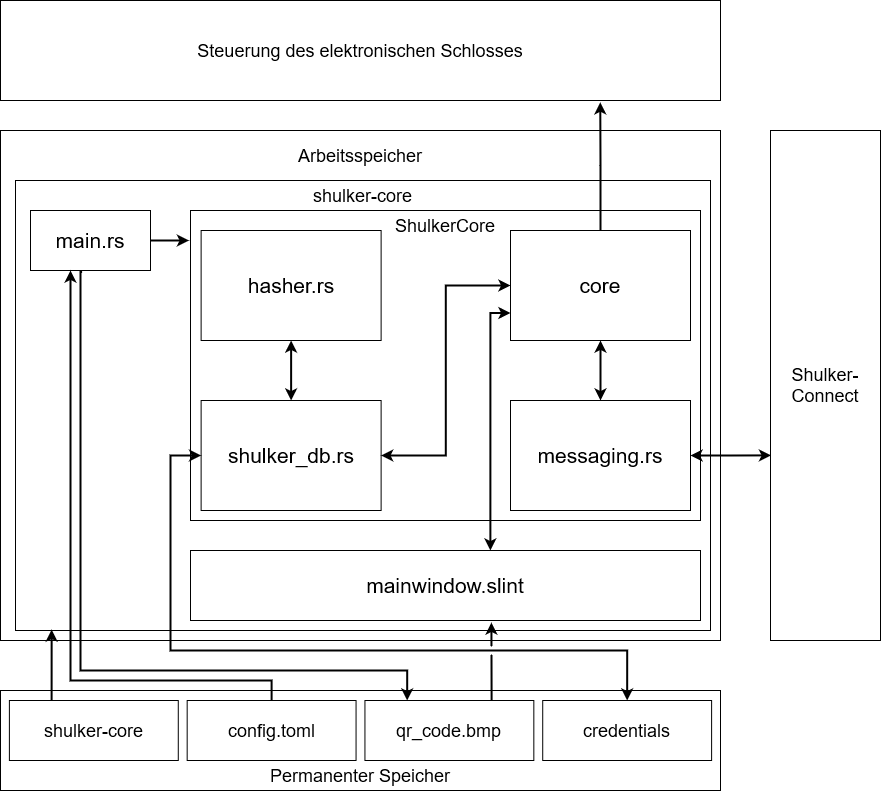
\includegraphics[width=0.8\textwidth]{images/core/informationsfluss.png}
        \caption{Informationsfluss in Shulker-Core}
    \end{center}
\end{figure}


\section{Konfiguration}
Die gesamte Konfiguration von Shulker-Core befindet sich in einer optionalen Textdatei. Da für jede mögliche Einstellung ein
Standartwert einprogrammiert ist, muss man nur nötige Änderungen vornehmen. Man muss sich also keine unnötigen Gedanken machen,
wie man jeden Wert in der Konfigurationsdatei definieren möchte.

Die Konfigurationsdatei hat das Dateiformat TOML und den Namen \textbf{config.toml}. Das Programm sucht im lokalen Ordner
nach dieser Datei. Das bedeutet, dass die config.toml-Datei sich im gleichen Ordner befinden muss, wie die Binary. Findet
Shulker-Core diese Datei nicht, werden alle Standartwerte übernommen. Als Warnung wird eine 
Warnmeldung an den Standart-Error ausgegeben.

\subsection{Mögliche Konfigurationen}
Es folgt eine Auflistung aller Konfigurationsschlüssel und ihrer Standartwerte:

\lstinline{master_password = "master123"}

Das Master-Passwort dient zur Identifikation der Admins. Das standartmäßige Adminpasswort sollte dringend durch 
ein Passwort vernünftiger Komplexität ersetzt werden. Es ist das einzige Passwort, das nicht gehashed wird. Dafür
gibt es drei Gründe: 
\begin{enumerate}
    \item Wer Zugriff zum Raspberry Pi hat, hat Zugriff zum Schloss.
    \item Dem Admin wird die Fähigkeit, ein einzigartiges Passwort zu erstellen, vorrausgesetzt.
    \item Bei Vergessen des Passworts kann der Admin es einfach wieder herausfinden. 
\end{enumerate}

\lstinline{send_socket_path = "/tmp/toShulkerServer.sock"}

Gibt den Pfad der Unix-Socket an, die zur Kommunikation mit Shulker-Connect dient; In Richtung Shulker-Core zu Shulker-Connect.
Um das System möglichst flexibel zu gestalten, wurde diese Konfiguration erschaffen. Man kann so leicht das System anpassen.

\lstinline{receive_socket_path = "/tmp/toShulkerCore.sock"}

Gibt den Pfad der Unix-Socket an, die zur Kommunikation mit Shulker-Connect dient; In Richtung Shulker-Connect zu Shulker-Core.
Um das System möglichst flexibel zu gestalten, wurde diese Konfiguration erschaffen. Man kann so leicht das System anpassen.

\lstinline{gpio_pin = 27}

Gibt an, welcher GPIO-Pin des Raspberries für die Ansteuerung des elektronischen Schlosses verwendet werden soll. Zu beachten:
soll das Schloss geschlossen sein, ist der GPIO-Pin auf High.

\lstinline{autolock_seconds = 24}

Die Dauer, die der GPIO-Pin bei richtiger Eingabe eines Pins (Passworts) auf High bleibt.

\lstinline{qr_code_link = "not setup!"}

Die Daten, die der QrCode in der M-Ansicht des Core-UIs enkodieren und zugänglich machen soll. Gedacht ist, dass der
Admin hier die IP des Raspberry Pis angibt.

\lstinline{hash_memory_size = 10}

Anzahl an Arbeitsspeicher, der für das Hashing der Pins verwendet wird. Genaueres wird später erklärt.

\lstinline{hash_iterations = 3}

Anzahl der Argon2id Durchläufe. Genaueres wird später erklärt.

\lstinline{hash_parallelism = 1}

Anzahl der Hash-Threads. Genaueres wird später erklärt.


\section{Abhängigkeiten}
Shulker-Core baut auf vielen \textit{crates}, also Codebibliotheken auf. Alle direkten Abhängigkeiten sind in der 
Cargo.toml-Datei nachvollziehbar. Es folgt eine kurze Auflistung und Erklärung der wichtigsten Abhängigkeiten:

\begin{itemize}
    \item \textbf{slint}; früher bekannt als SixtyFPS, ist ein User-Interface-Toolkit. Es ermöglicht relativ simples
    und plattformübergreifendes Programmieren von grafischen Benutzeroberflächen.

    \item \textbf{serde}; steht für \textbf{Ser}ialize und \textbf{De}serialize. Es ist das am bekannteste Framework,
    um Rust-Strukturen zu serialisieren und zu entserialisieren. Benutzt wird es, um die Kommunikation über Unix-Sockets zu
    ermöglichen.

    \item \textbf{argon2}; ist ein kryptographischer Passwort-Hashing Algorithmus. Das \textit{argon2}-crate implementiert diesen
    Algorithmus 100\%-ig mit Rust-Code. Die Variante Argon2id wird für das Unkenntlichmachen der Pins benutzt.

    \item \textbf{gpio-cdev}; wird verwendet, um den GPIO-Pin zu benutzen. Dabei wird auf die Linux-Kernel-API namens \textit{GPIO character device ABI}
    aufgebaut.

    \item \textbf{config}; ist ein crate, welches das Einlesen der Konfigurationsdatei erleichter.
    
    \item \textbf{chrono}; stellt Code zur Verfügung, um den Umgang mit Zeit und Datum zu erleichtern.
    
    \item \textbf{interprocess}; erleichtert die Verwendung von Unix-Sockets.
    
    \item \textbf{rustbreak}; eine einfache, in sich geschlossene Datenbank. Wird zur Speicherung von Daten verwendet.
    
    \item \textbf{qr\_code}; ermöglicht schnelles Erstellen von QrCodes. Wird verwendet um die Verbindung mit Shulker-Mobile zu
    erleichtern. Es ist das einzige crate, welches nicht von crates.io heruntergeladen wird. Das crate wird direkt von der Git-Repository auf
    Github kopiert.
\end{itemize}
\chapter{Der Touchscreen}
Der Touchscreen von Shulker kann grundsätzlich jeder Touchscreen mit akzeptabler Größe sein.
Die Steuerung des Touchscreens wird von Shulker-Core mithilfe des crates \textbf{slint} (Version 0.2) übernommen.

\section{Funktionsweise von slint}
Um mit slint eine grafische Benutzeroberfläche bereitstellen zu können, wird empfohlen, eine slint-Datei erstellen.
In dieser Datei wird mittels der .slint-Sprache eine Benutzeroberfläche beschrieben und programmiert. Diese Datei wird vom 
slint-Compiler in Binärcode umgewandelt. Da die .slint-Datei und der eigentliche Anwendungscode also getrennt sind, muss man sich
mittels Callbacks, Models und Eigenschaften verständigen. 
\begin{figure}[H]
    \begin{center}
        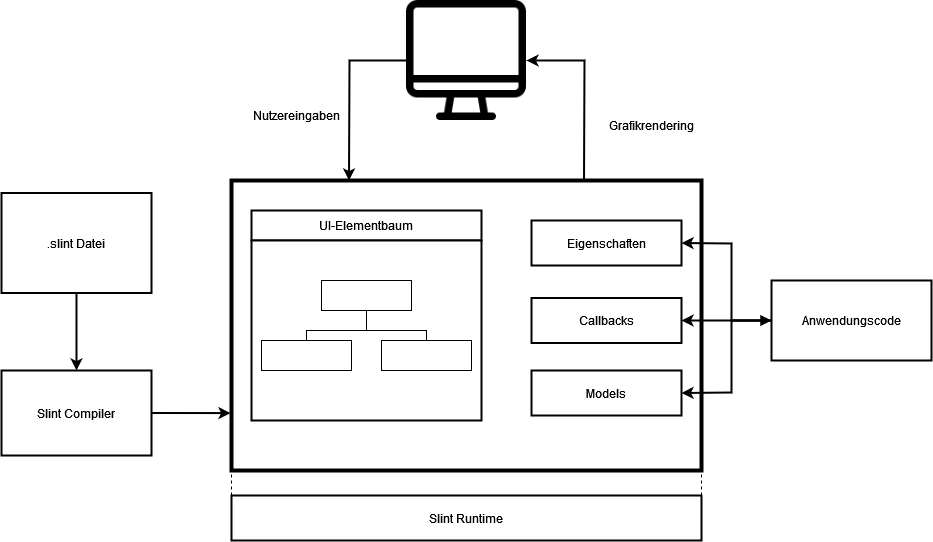
\includegraphics[width=0.9\textwidth]{images/core/slint_aufbau.png}
        \caption{Aufbau und Funktionsweise von slint}
    \end{center}
\end{figure}

\section{Aufbau der grafischen Oberfläche}
Shulker-Core verwendet eine .slint-Datei, welche den Namen \textit{mainwindow.slint} trägt. Diese Datei befindet sich im Unterordner
namens \textit{ui} in der Git-Repository von Shulker. Das Design der Oberfläche konzentriert sich darauf, möglichst leicht
lesbar und stromsparend zu sein. Deshalb entschieden wir uns für die Farben Schwarz und Weiß.

Die grafische Oberfläche besteht aus drei Teilen:
\begin{itemize}
    \item Menü-Selektor
    \item Hauptsicht
    \item Unlocked-Ansicht
\end{itemize}

\subsection{Menü-Selektor}
Der Menü-Selektor ist grundsätzlich immer zu sehen. Die einzige Ausnahme bildet das Entsperrtsein des elektronischen
Schlosses. Der Menü-Selektor ermöglicht das Wechseln der Hauptansicht. Es gibt drei Wahlmöglichkeiten:
\begin{itemize}
    \item \textbf{Pin}: zur Eingabe von Ziffernpins
    \item \textbf{PW}: zur Eingabe von Passwörtern, also Pins mit Buchstaben
    \item \textbf{M}: zur Verbindung mit Shulker-Mobile
\end{itemize}

\subsection{Hauptansicht}
Die Hauptansicht nimmt den Großteil des Bildschirms in Anspruch. In ihr wird dem Nutzer das Eingeben von Pins und Passwörtern
ermöglicht. Ein QR-Code zur Verbindung mit Shulker-Mobile lässt sich auch anzeigen.

\subsection{Unlocked-Ansicht}
Die Unlocked-Ansicht zeigt dem Nutzer, dass das Schloss momentan offen ist. Sie nimmt den ganzen Bildschirm in Anspruch und weicht
als einzige Komponente vom standart Farbschema ab; grelles Grün vermittelt ein klares Signal. Auf ihr ist auch ersichtlich,
wie lange das Schloss noch offen bleibt. Die Ansicht kann über mehrere Wege in den Vordergrund geschoben werden, grundsätzlich aber dann,
wenn an Shulker-Core ein Öffnen-Signal oder ein korrekter Pin gesendet wurde.

\chapter{Speicherung von Daten}
Shulker-Core speichert die vom Admin angelegten Pins ab. Alle Pins werden in einer Datei namens \textit{credentials} abgespeichert.
Es wird keine vollwertige Datenbank verwendet, um das System nicht zu groß zu gestalten und den Ressourcenverbrauch auf dem 
Raspberry möglichst gering zu halten.

\section{Rustbreak}
Shulker-Core verwendet das crate \textit{rustbreak} zum Speichern von Daten. Rustbreak ist eine von der Ruby-Datenbank \textit{daybreak} inspirierte
Datenbank, welche Daten nur in einer Datei speichert. Es wird die Version 2.0 von rustbreak verwendet.

Der große Vorteil von Rustbreak gegenüber einer herkömmlichen Datenbank ist, dass die gesamte Rustbreak-Datenbank in den
Arbeitsspeicher kopiert wird. Veränderungen an der Datenbank erfolgen dann im Arbeitsspeicher. Dem Programmierer ist es überlassen,
wann er die Datenbank im Arbeitsspeicher auf den permanenten Speicher überträgt und somit permanent abspeichert. Das ist von großen Vorteil,
da die meisten Raspberry Pi Setups eine sehr langsame SD-Karte als permanentes Speichermedium nutzen. Somit können Verzögerungen in der
Anwendung minimiert werden.

\section{Funktionsweise}
Shulker-Core lädt die gesamte \textit{credentials}-Datei beim Start in den Arbeitsspeicher. Wird ein eingegebener Pin
mit der Datenbank abgeglichen, muss so nur die geladene Datenbank abgefragt werden. Um Änderungen an der Datenbank permament zu 
machen, wird die geladene Datei nach jeder Änderung wieder auf die Festplatte kopiert. Das System ist so konfiguriert, dass
ein Fehler beim Abspeichern der Datei keine Probleme verursacht. Die Ursprungsdatei bleibt in solchen Fällen erhalten. Es kommt 
zu keinem Datenverlust.

\section{Hashing von Pins}
Da die Nutzer von Shulker aus Einfachkeit möglicherweise Passwörter nutzen wollen, die sie an anderen Orten bereits verwenden, werden
alle Pins gehashed abgespeichert. Somit ist es dem Admin und einem etwaigen Hacker nicht möglich, die originalen Pins nachzuvollziehen und
somit möglicherweise in anderen Bereichen Schaden anzurichten.

\subsection{Argon2}
Als Hashing-Algorithmus wird Argon2, genauer Argon2id verwendet. Argon2 wurde gewählt, da eine reine Rustimplementation des Algorithmus
existiert und der Algorithmus sich als Gewinner der \textit{Password Hashing Competition} herausgestellt hat.\cite{passwordhashingcmp}

\subsubsection{PHC-String}
Die unkenntlich gemachten Pins werden in der Form von PHC-Strings abgespeichert. Ein PHC-String besteht aus:
\begin{itemize}
    \item \textbf{id}: Kennzeichnung des verwendeten Hash-Algorithmus
    \item \textbf{version}: Version des Algorithmus
    \item \textbf{param}: mehrere Parameter, die dem Algorithmus gefüttert werden
    \item \textbf{salt}: zufällige Zeichenkette, welche das Schützen des Passworts weiter verbessert
    \item \textbf{hash}: der eigentliche Hash, also der unkenntlich gemachte Pin
\end{itemize}
\begin{figure}[H]
    \begin{center}
        
\includegraphics[width=1\textwidth]{images/core/phc_string.png}
        \caption{Beispiel eines PHC-Strings}
    \end{center}
\end{figure}
\cite{phcstring}

\subsubsection{Konfiguration von Argon2id}
Shulker-Core nimmt drei Parameter für Argon2id an:

\begin{itemize}
    \item \textbf{Memory}: Die Menge an Arbeitsspeicher, die der Algorithmus verwenden soll. Je höher dieser Wert ist,
    desto schwieriger ist es, den Hash nachzuvollziehen. Somit wird es einem Angreifer ebenfalls erschwert, viele Hashes zu generieren
    und somit das originale Passwort herauszufinden. Wird in der Shulker-Core-Konfigurationsdatei als \textit{hash\_memory\_size} definiert.
    \item \textbf{Iterations}: Wie oft sich der Algorithmus durch die ausgewählte Größe an Arbeitsspeicher durcharbeiten soll. Je höher, desto
    sicherer die Hashes. Wird in der Shulker-Core-Konfigurationsdatei als \textit{hash\_iterations} definiert.
    \item \textbf{Parallelism}: Wie viele Threads der Algorithmus verwenden soll. Desto höher dieser Wert, desto sicherer ist der Hash
    vor großen parallelen Attacken (zum Beispiel das Cracken mit Grafikkarten). Wird in der Shulker-Core-Konfigurationsdatei als \textit{hash\_parallelism} definiert.
\end{itemize}
\setcounter{secnumdepth}{1}
\appendix

\cleardoublepage
\phantomsection
\addcontentsline{toc}{chapter}{Literaturverzeichnis}
\bibliography{references} %references bibtech as used for all papers dealing with online-surveys
\nocite{*}

\cleardoublepage
\phantomsection
\addcontentsline{toc}{chapter}{\listfigurename}
\listoffigures
\cleardoublepage
\phantomsection
\addcontentsline{toc}{chapter}{Code-Snippet-Verzeichnis}
\listof{code}{Code-Snippet-Verzeichnis}

\end{document}